\documentclass[11pt]{article}
\usepackage[coverpage]{polytechnique}
\usepackage[utf8]{inputenc}     
\usepackage{amsmath}
\usepackage{amsfonts}
\usepackage[french]{babel}
\usepackage[version=3]{mhchem}
\usepackage{epstopdf}
\usepackage[justification=centering]{caption}
\usepackage{slashbox}
\usepackage[T1]{fontenc}
\usepackage{tikz}
\usetikzlibrary{arrows} 
\usepackage{pgfplots}
\usepackage[hidelinks]{hyperref}
\usepackage{subcaption}
\usepackage[version=3]{mhchem}
\usepackage{subcaption}
\usepackage{amsthm}
\usepackage{empheq}

\usepackage{geometry}

\newcommand*\widefbox[1]{\fbox{\hspace{2em}#1\hspace{2em}}}
\theoremstyle{definition}

\newtheorem{definition}{Définition}[section]

\theoremstyle{remark}
\newtheorem*{remark}{Remarque}


\title{Enseignement d'Approfondissement}
\date{Décembre-Février 2016}
\author{Dhruv SHARMA \\ José MORAN}
\subtitle{Simulation d'un système bosonique avec des intégrales de chemin}

\newcommand{\hham}{\hat{H}}
\newcommand{\dom}{L\mathbb{T}^d}
\begin{document}
\maketitle
\newpage
\tableofcontents
\newpage
\section*{Introduction}
Dans cet EA nous nous sommes intéressés à différentes méthodes 


\newpage
\section{Fonction de partition d'un système quantique}\label{sec:part}
On se propose d'étudier un système équivalent à deux particules identiques (même masse donc) dans une boîte à $d$ dimensions, par exemple deux particules dans la boîte $[0;1]^d$ avec des conditions périodiques et l'hamiltonien :
\begin{equation}
\hham = -\frac{\hbar^2}{2m}\sum_{i=1}^{d}\left( \frac{\partial^2}{\partial x_{1,i}}+\frac{\partial^2}{\partial x_{2,i}}\right)+v(x_1)+v(x_2)+w(x_1,x_2)
\end{equation}

où $v$ est le potentiel à une particule et $w$ le potentiel d'interaction à deux particules, supposés ici continus. On pourra, par exemple, s'intéresser à la dynamique du système si on prend pour $v$ un potentiel avec deux puits de profondeurs inégales, et étudier dans quel cas les deux particules sont dans le même puits et dans quel cas elles sont dans des puits différents.
\\

Dans le cas général, nous étudions le système de $N$ particules dans un domaine que nous appelons $\dom$, où $L$ est la longueur caractéristique du domaine et $d$ sa dimension. Nous verrons après qu'il convient de prendre un tore.
\\

Dans ce cas, nous avons toujours au minimum $\hham$ autoadjoint sur $\mathcal{H}=\mathrm{L}^2(\dom)$. Pour étudier notre système nous avons par ailleurs besoin de définir pour $\beta = \frac{1}{k_BT}\geq 0$ l'opérateur :
\begin{equation}
\hat{A}(\beta)=e^{-\beta \hham}
\end{equation} 
Comme $\hham$ est autoadjoint, cet opérateur est un opérateur auto-adjoint positif. Par ailleurs nous avons que 
\begin{equation}
Z(\beta)=\mathrm{Tr}(\hat{A}(\beta))=\mathrm{Tr}(e^{-\beta \hham})\in \mathbb{R}^+\cup \lbrace+\infty\rbrace
\end{equation}
Pour que $Z(\beta)\in\mathbb{R}^+$ il faut que $\hham$ soit borné inférieurement et à résolvante compacte. Dans la pratique, deux cas de figure suffissent à avoir cela :
\begin{itemize}
\item on prend pour $v$ un potentiel confinant et pour $w$ un potentiel borné.
\item le domaine correspond à une super-cellule, i.e. on prend un tore (conditions aux bords périodiques).
\end{itemize}
Nous allons donc considérer pour $\dom$ le tore de longueur caractéristique $L$ et de dimension $d$.
Nous pouvons alors dans ce cas général à N particules écrire un hamiltonien où nous séparons la partie cinétique de la partie potentielle :
\begin{equation}
\hham_N=\hat{T}_N+\hat{V}_N ,
\end{equation}
où, en notant $X=(x_1,x_2,...,x_{N-1},x_N)$ le vecteur à $dN$ composantes : 
\begin{equation}
\hat{T}_N=-\frac{\hbar^2}{2m}\sum_{i=1}^{N}\Delta_{x_i}=-\frac{\hbar^2}{2m}\Delta_X
\end{equation}
est l'énergie cinétique des $N$ particules.
De même nous allons nous restreindre, du moins dans un premier temps, au cas où nous n'avons que le potentiel agissant sur chaque particule et le potentiel d'intéraction entre deux particules, c'est-à-dire : 
\begin{equation}
\hat{V}_N=\sum_{i=1}^N v(x_i)+\sum_{1\leq i < j \leq N} w(x_i,x_j)
\end{equation}
Ainsi si nous prenons $v$ et $w$ bornées à valeurs réelles, alors $\hham_N$ est auto-adjoint, borné inférieurement, à résolvante compacte et la fonction de partition $Z(\beta)$ est bien définie car nous avons que 
\begin{equation}
\forall \beta>0,\quad Z(\beta)<\infty
\end{equation}

Notre objectif pour la suite sera d'exprimer la fonction de partition comme une intégrale.
\subsection{Expression de $Z$ comme une intégrale}
Soit $\beta>0$ fixé. Alors, comme vu auparavant, $e^{-\beta\hham}$ est un opérateur à trace. Nous savons par ailleurs qu'il a un noyau $k_{\beta}(X,X'), (X,X')\in(\dom)^2$, i.e. que pour tout $\psi\in \mathcal{H}$:
\begin{equation}
(e^{-\beta \hham}\psi)(X)=\int_{\dom} k_{\beta}(X,X')\phi(X')\mathrm{d}X'.
\end{equation}
Il est possible, par des arguments de régularité elliptiques, de montrer que $k_\beta$ est une fonction régulière.
On peut ainsi montrer que dans ce cas :
\begin{equation}
Z(\beta)=\mathrm{Tr}(e^{-\beta \hham})=\int_{\dom}k_\beta(X,X)\mathrm{d}X
\end{equation}
Nous allons donc exprimer ceci à l'aide de la formule de Trotter, qui dit que, pour $\hham=\hat{V}+\hat{T}$ :
\begin{equation}
(e^{-\beta \hham}\psi)(X)=\lim_{M\to \infty}\left[(e^{-\frac{\beta}{2M}\hat{V}}e^{-\frac{\beta}{M}\hat{T}}e^{-\frac{\beta}{2M}\hat{V}})^M\psi\right](X),
\end{equation}
Où la limite s'entend au sens de $\mathrm{L}^2$. 

\subsection{Démonstration de la formule de Trotter}
Nous notons dorénavant $V=\hat{V}$ et $T=\hat{T}$.
Nous avons pour M quelconque les égalités suivantes : 
\begin{equation}
(e^{-\frac{\beta}{2M}V}\psi)(X)=e^{-\frac{\beta}{2M}V(X)}\psi(X)
\end{equation}
\begin{align}
(e^{-\frac{\beta}{M}T}\psi)(X)&=(e^{\frac{\hbar^2\beta}{2mM}\Delta}\psi)(X)\\
&=\int_{\dom}k_T(X,X')\psi(X')\mathrm{d}X'
\end{align}
où nous avons noté, avec $\sigma^2=\frac{mM}{\beta \hbar^2}$, 

\begin{equation}
k_T(X,X')=\sum_{k\in\mathbb{Z}^{dN}}\frac{1}{(2\pi\sigma^2)^{\frac{dN}{2}}}\exp\left(-\frac{|X-X'-k|^2}{2\sigma^2}\right).
\end{equation}
Or pour $\sigma$ petit, i.e. pour $M$ grand, seul le terme en $k=0$ a une contribution appréciable, de sorte que, lorsque $M\gg 1$: 
\begin{equation}
k_T(X,X')\simeq\frac{1}{(2\pi\sigma^2)^{\frac{dN}{2}}}e^{-\frac{|X-X'|^2}{2\sigma^2}}
\end{equation}


Posons 
\begin{equation}
h_M=e^{-\frac{\beta}{2M}\hat{V}}e^{-\frac{\beta}{M}\hat{T}}e^{-\frac{\beta}{2M}\hat{V}}
\end{equation}

Ainsi 
\begin{align*}
(h_M^M\psi)(X) &=  e^{-\frac{\beta}{2M}V(X)}\int_{\dom}k_T(X,X_1)e^{-\frac{\beta}{2M}}V(X_1)\left(h_M^{M-1}\psi\right)(X_1)\mathrm{d}X_1
\\
&= e^{-\frac{\beta}{2M}V(X)}\int_{(\dom)^2}k_T(X,X_2)k_T(X_2,X_1)e^{-\frac{\beta}{M}\left(V(X_2)+\frac{V(X_1)}{2}\right)}\left(h_M^{M-2}\psi\right)(X_1)\mathrm{d}X_1\mathrm{d}X_2
\\
&=e^{-\frac{\beta}{2M}V(X)}\int_{(\dom)^3}k_T(X,X_3)k_T(X_3,X_2)k_T(X_2,X_1)e^{-\frac{\beta}{M}\left(V(X_3)+V(X_2)+\frac{V(X_1)}{2}\right)}\left(h_M^{M-3}\psi\right)(X_1)\mathrm{d}X_1 \\ 
&\mathrm{d}X_2 \mathrm{d}X_3
\\
&\vdots
\\
&=e^{-\frac{\beta}{2M}V(X)} \int_{(\dom)^{M-1}} \left(\prod_{i=1}^{M-1}\mathrm{d}X_i\right)k_T(X,X_{M-1})\ldots k_T(X_2,X_1) e^{-\frac{\beta}{M}\left(\frac{V(X_1)}{2}+\sum_{i=2}^{M-1}V(X_i)\right)}\\ &\left(h_M\psi\right)(X_1)
\\
&= e^{-\frac{\beta}{2M}V(X)}\int_{(\dom)^{M}}\left(\prod_{i=1}^{M}\mathrm{d}X_i\right) k_T(X,X_{M})\ldots k_T(X_2,X_1) e^{-\frac{\beta}{M}\left(\frac{V(X_1)}{2}+\sum_{i=2}^{M}V(X_i)\right)}\psi(X_1)
\\
&=\frac{1}{(2\pi\sigma^2)^\frac{dNM}{2}}\int_{(\dom)^M} \left(\prod_{i=1}^{M}\mathrm{d}X_i\right) e^{-\frac{1}{2\sigma^2}\sum_{i=1}^{M}|X_{i+1}-X_i|^2-\frac{\beta}{M}\left(\frac{V(X_{M+1})+V(X_1)}{2}+\sum_{i=2}^{M}V(X_i)\right)}\psi(X_1)
\\
&=\frac{1}{(2\pi\sigma^2)^\frac{dNM}{2}}\int_{(\dom)^M} \left(\prod_{i=1}^{M}\mathrm{d}X_i\right) e^{-\beta \mathcal{V}(X,X_1,\ldots,X_M)}\psi(X_1),
\end{align*}

où l'on a posé $X_0=X$ et :
\begin{equation}
\mathcal{V}\left(X_0,X_1,\ldots,X_M\right)= \frac{1}{2\beta\sigma^2}\sum_{i=0}^{M-1}|X_{i+1}-X_i|^2+\frac{1}{M}\left(\frac{V(X_0)+V(X_1)}{2}+\sum_{i=1}^{M-1} V(X_i)\right)
\end{equation}

$\mathcal{V}$ s'interprête comme l'énergie potentielle de $M+1$ systèmes à $N$ particules, où les particules intéragissent entre elles au sein d'un même système, comme on le voit dans la somme des $V(X_i)$, et d'un système au suivant avec elles mêmes, à travers le terme en $\sum \frac{|X_{i}-X_{i+1}|^2}{2\beta\sigma^2}$.

Ainsi nous avons immédiatement que 
\begin{equation}
(h_M^M\phi)(X)=\int_{\dom}k_h(X,X')\mathrm{d}X'
\end{equation}
Avec 
\begin{equation}
k_h(X,X')=\frac{1}{(2\pi\sigma^2)^\frac{dNM}{2}}\int_{(\dom)^{M-1}} \left(\prod_{i=1}^{M-1}\mathrm{d}X_i\right) e^{-\beta \mathcal{V}(X,X_1,\ldots,X_{M-1},X')}
\end{equation}

Nous pouvons enfin calculer la fonction de partition du système pour $M$ suffisament grand :
\begin{align*}
Z(\beta)=\mathrm{Tr}(e^{-\beta H})& \simeq \mathrm{Tr}(h_M^M)
\\
&= \int_{\dom}\mathrm{d}X k_h(X,X)
\\
&= \frac{1}{(2\pi\sigma^2)^\frac{dNM}{2}}\int_{(\dom)^{M}} \mathrm{d}X\left(\prod_{i=2}^{M}\mathrm{d}X_i\right) e^{-\beta S_M(X,X_M,\ldots,X)}
\end{align*}

Où l'intégrale ci-dessus s'interprète comme l'intégrale de la pseudo-action $S_M$ le long d'un chemin qui part de $X$ et revient vers $X$ en temps $\beta$ fini.

\section{Mouvement Brownien, Calcul d'Itô et formule de Feynman-Kac}\label{sec:brown}
Dans cette partie nous décrirons une méthode probabiliste pour évaluer le noyau $k_{\beta}$ que nous avons décrit dans la section précédente. 
Avant de commencer le calcul de $k_{\beta}$, nous allons introduire quelques notions utiles.

\subsection{Definitions}

\theoremstyle{definition}

\begin{definition}{\textbf{Processus de Markov}}

Soit $(X_n)_{n >0}$ un processus aléatoire discret sur un espace d'états dénombrable $E$. Le processuss satisfait la propriété de Markov si pour toute collection d'états $(x_0, x_1, ... x_n) \in E$, nous avons 

\begin{equation} 
\mathbb{P}(X_{n+1} = y | X_0 = x_0, X_1 = x_1,....X_n = x_n) = \mathbb{P}(X_{n+1} = y | X_n = x_n)
\end{equation}

Il faut que les deux probabilités conditionnelles soient bien définies. Le processus $(X_n)_{n>0} $ est alors appelé un processus de Markov.

\end{definition}

\begin{definition}{\textbf{Ergodicité}}

Un processus est ergodique s'il satisfait les conditions suivantes :

\begin{itemize}

\item 

$\varphi$ est une mesure de probabilité invariante par le processus de Markov. 

\item 

\textbf{Condition d'accessibilité}: 

\begin{align}
\forall \mathrm{B} \in \mathcal{B}(\mathbb{R}^d)\quad \mathrm{t.q.}\quad \varphi(\mathrm{B})>0, \quad \forall x\in\mathbb{R}^d, \quad \exists n\in\mathbb{N} \quad \mathrm{t.q.}\quad \mathbb{P}(\mathrm{X}_n \in \mathcal{B} | \mathrm{X}_0 =n ) > 0 
\end{align}
\end{itemize}

\end{definition}

\begin{remark}
\begin{enumerate}
\item 
Nous avons défini la notion d'ergodicité sur $\mathbb{R}^d$, mais les mêmes définitions restent valables pour $\mathrm{L}\mathbb{T}^d$.
\item 
Au moment de simuler avec l'algorithme de Metropolis, il suffira de vérifier que la probabilité de transfert pour cet algorithme satisfait la condition d'accessibilité dans la définition d'ergodicité.

\end{enumerate}
\end{remark}


\begin{definition}{\textbf{Chaînes de Markov}}

Une chaîne de Markov (discrète) est un processus de Markov défini par :

\begin{equation}
\left\{ 
  \begin{array}{ll}
  \mathrm{X}_{n+1}^{\Delta t} &= \mathrm{X}_{n}^{\Delta t} + b(\mathrm{X}_{n}^{\Delta t}) + \sqrt{\Delta t} \xi_{n}
  \\
  \mathrm{X}_{0}^{\Delta t} &\sim  f(x) \mathrm{d}x 
  \end{array}
\right.
\end{equation}



avec $x \in \mathbb{R}^d$ et $b: \mathbb{R}^d \to \mathbb{R}^d$ une fonction régulière. Ici $\xi_{j} \sim \mathcal{N}(0,1)_{\mathbb{R}^d}$, i.e. $\xi_{j}$ est un vecteur gaussien de dimension $d$. 
\end{definition}

À partir de la chaine de Markov defini ci-dessus nous pouvons construire un processus de Markov en temps continu en reliant les instants de temps $t_n$ et $t_{n+1}$ de manière affine. Dans ce cas, nous avons avec les mêmes conditions que ci-dessus :

\begin{align}
\forall t \in [t_n,t_{n+1}],\quad\tilde{\mathrm{X}}_{t}^{\Delta t} &= \mathrm{X}_{n}^{\Delta t} + (t-t_n) \mathrm{X}_{n+1}^{\Delta t} 
\end{align}

Nous avons de même 
\begin{equation}
\tilde{\mathrm{X}}_{t}^{\Delta t} \underset{\Delta t \to 0}{\longrightarrow} \mathrm{X}_t
\end{equation}


où $\mathrm{X}_{t}$ suit l’équation différentielle stochastique donnée par: 

\begin{align}
\label{equ_stoch_x}
\mathrm{dX}_{t} &= b(\mathrm{X}_{t})\mathrm{d}t + \mathrm{dW}_{t} \\
\mathrm{X}_{0} &\sim f(x)\mathrm{d}x
\end{align}

où $\mathrm{W}_{t}$ est le processus de Wiener.

\subsection{Formule d'Itô}

A la fin de la section précédente, nous avons abouti à une équation différentielle stochastique qui détermine le processus de Markov en temps continu. Pour faciliter la résolution de cette équation, nous  mettrons en place des formules de calcul différentiel stochastique qui nous permettront d'aboutir à la formule de Feynman-Kac. 

Considérons d'abord l’équation \eqref{equ_stoch_x} sans le terme stochastique $\mathrm{dW}_{t}$. Dans ce cas, l'équation devient déterministe et sa solution $\mathrm{Y}_t$ suit l'équation:

\begin{equation}
\frac{\mathrm{dY}_{t}}{\mathrm{d}t} = b(\mathrm{Y}_t) 
\end{equation}

Pour rester dans un cadre simple, nous travaillerons dans $\mathbb{R}$, mais les résultats sont bien évidemment généralisables sur $\mathbb{R}^d$. Soit $h: t \times \mathbb{R}^d \rightarrow \mathbb{R}$. Alors nous avons : 

\begin{align*}
\mathrm{d}(h(\mathrm{Y}_{t})) &= \frac{\partial h}{\partial t}(t,\mathrm{Y}(t)) \mathrm{d}t + \nabla h(\mathrm{Y}_{t}) \mathrm{dY}_{t} \\
&= \frac{\partial h}{\partial t}(t,\mathrm{Y}(t)) \mathrm{d}t + \nabla h(\mathrm{Y}_{t}) b(\mathrm{Y}_{t})\mathrm{d}t
\end{align*}

Dans le cas de $\mathrm{X}_{t}$, solution de l'équation différentielle stochastique \eqref{equ_stoch_x}, la différentielle de $h(t, \mathrm{X}_t)$ contient un terme supplémentaire faisant intervenir les dérivées secondes de h. Nous obtenons finalement:

\begin{equation}
\mathrm{d}(h(t,\mathrm{X}_t)) = ( \frac{\partial h}{\partial t}(t, \mathrm{X}_t) + \nabla h(t,\mathrm{X}_t) b(\mathrm{X}_t) + \frac{1}{2} \Delta h(t,\mathrm{X}_t) )\mathrm{d}t + \nabla h(t,\mathrm{X}_t) \mathrm{dW}_{t}
\end{equation}

\subsection{Le Formule de Feynman-Kac}

Munis des règles du calcul différentiel, nous sommes maintenant en mesure de dériver la formule de Feynman-Kac.

Pour ce faire, nous introduisons deux équations : les équations de Kolmogorov forward et backward.

\begin{definition}{\textbf{L'equation de Kolmogorov forward}}
C'est une équation différentielle associé à \eqref{equ_stoch_x} définie  dans $]0,\beta] \times \Omega$ par : 

%Il faut expliciter le domaine, j'imagine ? Ou la classe de u ? 
\begin{equation}
\label{kolmo_forw}
\begin{split}
\frac{\partial u}{\partial t} &= \frac{1}{2} \Delta u - \mathrm{div}(bu) - \mathrm{V}u \\
u(0) &= f(x)
\end{split}
\end{equation}

\end{definition}



\begin{definition}{\textbf{L'équation de Kolmogorov backward}}

Dans $]0,\beta] \times \Omega$, nous definissons l'equation de Kolmogorov backward associé à \eqref{equ_stoch_x}

\begin{equation}
\label{kolmo_back}
\begin{split}
\frac{\partial v}{\partial t} + \frac{1}{2} \Delta v + b \nabla v - \mathrm{V}v &= 0 \\
v(\beta, x) &= g(x)
\end{split}
\end{equation}
\end{definition}

Nous considérons la dérivée totale $\mathrm{d}(v(t, \mathrm{X}_{t}) e^{-\int_0^{t} \mathrm{V}(\mathrm{X}_{s}) \mathrm{d}s})$ où $\mathrm{X}_{t}$ est défini en \eqref{define_xt}. En utilisant l'équation \eqref{develop_ito_x}, nous trouvons que :

\begin{multline}
\begin{split}
\mathrm{d}(v(t, \mathrm{X}_{t}) e^{-\int_0^{t} \mathrm{V}(\mathrm{X}_{s}) \mathrm{d}s}) = (\frac{\partial v}{\partial t} + b \nabla v + \frac{1}{2}\Delta v - \mathrm{V}v)e^{-\int_0^{t} \mathrm{V}(\mathrm{X}_{s}) \mathrm{d}s} \\
+ \nabla v(t, \mathrm{X}_t)\mathrm{dW}_{t} e^{-\int_0^{t} \mathrm{V}(\mathrm{X}_{s}) \mathrm{d}s}
\end{split}
\end{multline}

et le premier terme est nul d'après \eqref{kolmo_back}. Donc :

\begin{align}
\mathrm{d}(v(t, \mathrm{X}_{t}) e^{-\int_0^{t} \mathrm{V}(\mathrm{X}_{s}) \mathrm{d}s}) = \nabla v(t, \mathrm{X}_t)\mathrm{dW}_{t} e^{-\int_0^{t} \mathrm{V}(\mathrm{X}_{s}) \mathrm{d}s}
\end{align}

Enfin nous remarquons que l’espérance de $\nabla v(t, \mathrm{X}_t)\mathrm{dW}_{t} e^{-\int_0^{t} \mathrm{V}(\mathrm{X}_{s}) \mathrm{d}s}$ est nulle, et en utilisant la commutation des différentes opérations avec l’espérance, nous avons ainsi que: 

\begin{align}
\mathbb{E}(v(t , \mathrm{X}_{t})e^{-\int_0^{t} \mathrm{V}(\mathrm{X}_{s}}) = \mathrm{cte}
\end{align}

En particulier:

\begin{align}
\mathbb{E}(v(\beta , \mathrm{X}_{\beta})e^{-\int_0^{\beta} \mathrm{V}(\mathrm{X}_{s})}) &= \mathbb{E}(v(0, \mathrm{X}_0)), \\
\mathbb{E}(g(x_{\beta}))e^{-\int_0^{\beta} \mathrm{V}(\mathrm{X}_{s})}) &= \int_{\Omega} v(0,x) f(x) \mathrm{d}x.
\end{align}

où nous avons utilisé la condition initiale de \eqref{kolmo_back} et où l’intégration porte sur l'ouvert $\Omega$ considéré. 

Considérons maintenant l'intégrale $\int_{\Omega} v(0,x) f(x) \mathrm{d}x$. Par la condition initiale de \eqref{kolmo_forw}, nous avons par conséquent :

\begin{equation}
\int_{\Omega} v(0,x) f(x) \mathrm{d}x = \int_{\Omega} v(0,x) u(0,x) \mathrm{d}x
\end{equation}

D'où:

\begin{align}
\label{expansion_integral_vu}
\begin{split}
\int_{\Omega} v(0,x) u(0,x) \mathrm{d}x &= \int_{\Omega} v(\beta, x) u(\beta,x) \mathrm{d}x - \int_{0}^{\beta} \frac{\mathrm{d}}{\mathrm{d}t}\left(\int_{\Omega} v(t,x) u(t,x) \mathrm{d}x \right) \mathrm{d}t \\
&= \int_{\Omega} v(\beta, x) u(\beta,x) \mathrm{d}x - \int_{0}^{\beta} \left( \int_{\Omega} \frac{\partial v}{\partial t} u \mathrm{d}x + \frac{\partial u}{\partial v} \mathrm{d}x \right) \mathrm{d}t
\end{split}
\end{align}

Nous remarquons alors que les problèmes \eqref{kolmo_forw} et \eqref{kolmo_back} sont l'adjoint l'un de l'autre pour le produit scalaire usuelle defini pour l'espace $\mathrm{L}^2$. En d'autres termes, si $L$ est un opérateur différentiel et $L^{*}$ son opérateur adjoint, nous avons : 

\begin{align}
\label{adjoint_conditions}
\begin{split}
\frac{\partial u}{\partial t} &= \mathrm{L}u  \\
\frac{\partial v}{\partial t} &= -\mathrm{L}^{*}v
\end{split}
\end{align}

En d'autres termes :
\begin{align}
- \int_{0}^{\beta} \left( \int_{\Omega} \frac{\partial v}{\partial t} u \mathrm{d}x + \frac{\partial u}{\partial v} \mathrm{d}x \right) \mathrm{d}t &= 
- \int_{0}^{\beta} \left( (-L^{*}v,u)_{\mathrm{L}^2} + (v, Lu)_{L^2} \right) \mathrm{d}t &= 0
\end{align}

Ainsi :

\begin{align*}
\int_{\Omega} v(\beta, x) u(\beta, x) \mathrm{d}x &= \int_{\Omega} v(0,x) f(x) \mathrm{d}x \\
\int_{\Omega} g(x) u(\beta, x) \mathrm{d}x &= \int_{\Omega} v(0,x) f(x) \mathrm{d}x
\end{align*}

et on déduit la formule de Feynman-Kac : 

\begin{empheq}[box=\widefbox]{align}
\label{feynman_kac}
\int_{\Omega} g(x) u(\beta,x) \mathrm{d}x &= \mathbb{E}\left( g(x_{\beta}) e^{-\int_{0}^{\beta} \mathrm{V}(x_s)\mathrm{d}s} \right)
\end{empheq}

où $\mathrm{X}_{t}$ est la solution de \eqref{equ_stoch_x}

\subsection{Application à notre problème} 

Revenons sur notre problème de départ, qui est de trouver le noyau de l'opérateur $e^{-\beta H}$. Nous rappelons que le noyau est une fonction $k_{\beta}$ telle que:

\begin{equation}
\label{def_noyau} 
\left(e^{-\beta H} f \right)(x) = \int_{\Omega} k_{\beta}(x,y) f(y) \mathrm{d}y
\end{equation}

Nous remarquons que, pour $b=0$, $e^{-\beta H} f$ est la solution de \eqref{kolmo_forw}. D'où en appliquant \eqref{feynman_kac} :

\begin{equation}
\int_{\Omega X \Omega} k_{\beta}(x,y) f(y)g(x) \mathrm{d}x\mathrm{d}y = \mathbb{E}\left( g(\mathrm{X}_{\beta}) e^{-\int_{0}^{\beta} \mathrm{V}(\mathrm{X}_s)\mathrm{d}s} \right)
\end{equation}

où $\mathrm{X}_t$ est la solution de \eqref{equ_stoch_x}. 

Cette dernière condition étant vraie pour tout $f$, nous prenons $f(y) = \delta(y)$, le delta de Dirac. Dans ce cas, nous avons pour le processus $\mathrm{X}_{t}$ : 
\begin{equation}
\mathrm{X}_{\beta} = y + \mathrm{W}_{\beta}
\end{equation}. 

D'où:

\begin{align}
\begin{split}
\int_{\Omega} k_{\beta}(x,y) g(x) \mathrm{d}x &= \mathbb{E}\left( g(y+\mathrm{W}_{\beta}) e^{-\int_{0}^{\beta} V(y+\mathrm{W}_s) \mathrm{d}s} \right) \\
&= \int_{\Omega} g(x) \mathbb{E}_{y+\mathrm{W}_{\beta}=x} \left( e^{-\int_{0}^{\beta} V(y+\mathrm{W}_{s}) \mathrm{d}s} \right) \mathrm{d}x
\end{split}
\end{align}

Nous identifions alors le noyau comme étant : 

\begin{empheq}[box=\widefbox]{align}
\label{noyau_esperance}
k_{\beta}(x,y) = \mathbb{E}_{y+\mathrm{W}_{\beta}=x} \left( e^{-\int_{0}^{\beta} V(y+\mathrm{W}_{s}) \mathrm{d}s} \right)
\end{empheq}

Dans notre cas, nous nous intéressons au calcul de la fonction de partition $Z = \mathrm{Tr}(e^{-\beta H})$, qui d'après ce qui précède s'écrit : 

\begin{align}
\label{partition_func_martingale}
\begin{split}
Z &= \mathrm{Tr}(e^{-\beta H}) = \int_{\Omega} k_{\beta}(x,x) \mathrm{d}x \\
&= \int_{\Omega} \mathbb{E}_{\mathrm{W}_{\beta} =0} \left( e^{-\int_{0}^{\beta} V(x+\mathrm{W}_{s})} \right)
\end{split}
\end{align}

\begin{remark}
Nous devons interpréter les deux termes dans cette dernière relation. Prenons d'abord $\mathbb{E}_{\mathrm{W}_{\beta=0}}$. C'est le terme d’espérance sur les ponts browniens, c'est-à-dire une espérance sur tous les chemins allant de $x_0$ au temps $t=0$ jusqu'au un temps $\beta$ où l'on revient au point de départ $x_{\beta}=x_0$. 

Le deuxième terme en exponentielle représente la création ou annihilation des particules à un point $x+\mathrm{W}_{s}$ donné. Nous formons donc une image de ce processus comme suivant : 

\begin{enumerate} 

\item 

Le particule commence son trajet à $x_{t=0}=x_0 = 0$. Nous allons regarder seulement les trajets qui finissent à un temps $t=\beta$, de sorte que $x_\beta = 0$.

\item 

Pendant ce trajet, la particule peut être détruite ou créée selon le poids probabiliste $e^{-\int_{0}^{\beta} V(x+\mathrm{W}_{s})}$. 

\item 

L’espérance sur tous ces trajets nous donne la fonction de partition $Z = \mathrm{Tr}(e^{-\beta H})$. 
\end{enumerate}


\end{remark}

\section{Les Systèmes Bosoniques}\label{sec:bosons}

Les systèmes bosoniques sont les systèmes quantiques constitué par des bosons. Les bosons sont des particules dont le spin est entier, par opposition aux fermions, dont le spin est demi-entier. Le théorème de spin-statistique, dont les implications seront expliquées dans la suite, engendre des comportements très différents entre les systèmes bosoniques et fermioniques.

En effet en mécanique quantique, l'état d'un système est décrit par un vecteur d'état $|\psi \rangle$, qui contient toute l'information du système. Cet état évolue selon la fameuse équation de Schroedinger. Le fait que les bosons ont un spin entier et les fermions un spin demi-entier a des implications sur les propriétés de $| \psi \rangle$. En effet lorsqu'on considère $N$ particules, l'état total du système est noté :
\begin{equation}
|\psi^{(1)},\psi^{(2)},\ldots,\psi^{(N)}\rangle
\end{equation}

On considère alors l'opérateur $P_{ij}$ qui échange les particules $i$ et $j$. Il s'agit d'un opérateur auto-adjoint, et il est évident que $P_{ij}^2=1$. Les valeurs propres de $P_{ij}$ sont alors $\pm 1$. Le théorème de spin-statistique nous assure alors que $P_{ij}=1$ pour les bosons et $P_{ij}=-1$ pour les fermions.

En particulier, l’état décrivant un système de $N$ bosons est symétrique par échange de deux particules tandis qu'il est antisymétrique pour des fermions. C'est-à-dire que pour les états de $N$ bosons ou de $N$ fermions peuvent être écrits de la manière suivante : 

\begin{align} 
\label{symetrie_boson_fermion}
|\psi^{(1)},\psi^{(2)},\ldots,\psi^{(N)}\rangle_B &= \sqrt{\frac{1}{N!}} \sum_P |\psi^{P(1)},\psi^{P(2)},\ldots,\psi^{P(N)}\rangle \\
|\psi^{(1)},\psi^{(2)},\ldots,\psi^{(N)}\rangle_F &= \frac{1}{\sqrt{N!}} \sum_P \sigma (P) |\psi^{P(1)},\psi^{P(2)},\ldots,\psi^{P(N)}\rangle
\end{align}

où $B$ est pour les bosons, $F$ pour les fermions. Ici la somme porte sur touts les états possible sous une permutation $P$ de $\left\lbrace 1\ldots N\right\rbrace$. La racine est prise afin de normaliser l'état. Finalement, $\sigma (P)$ est la signature de la permutation $P$ (+1 si $P$ contient un nombre paire de transpositions et -1 sinon). 

Vu qu'un état complet d'un système bosonique contient tous les permutations possible de $N$ particules, nous devons prendre en compte cette symétrie dans notre modélisation des systèmes bosoniques par une intégrale de chemin. Concrètement, cela implique que pour un système des bosons, la matrice densité s'écrit de la manière suivante: 

\begin{align} 
\label{densite_boson}
\rho_{B}( \mathbf{X}, \mathbf{X}'; \beta) = \frac{1}{N!}\sum_{\mathcal{P}} \rho_{D} (\mathbf{X}, P \mathbf{X}'; \beta)
\end{align}

où $\rho_{D}$ est la matrice densité pour un système de $N$ particules discernables. Pour des particules discernables, des particules classiques par exemple, nous pouvons commencer avec un ensemble des points $\mathbf{X}$ donné et retourner à ce même point. Cependant, pour les particules comme des bosons(ou des fermions), nous pouvons arriver vers un point $P\mathbf{X}$, c'est-à-dire une permutation de l'ensemble $\mathbf{X}$. Ainsi, en effectuant un calcul d’intégrale de chemin pour un système bosonique, nous devons sommer non seulement sur tous les chemins allant du point $X$ à $X'$, mais sur tous les chemins partant de $X$ et arrivant en $PX'$. Cela fait à la fois la richesse du comportement des bosons mais aussi la difficulté technique à laquelle nous devons faire face. 

\section{Méthodes numériques}\label{sec:num}
\subsection{L'algorithme Métropolis}\label{ssec:metropolis}

Un outil indispensable pour toutes les méthodes de Monte-Carlo est l'algorithme de Metropolis que nous allons décrire ici. 

L'algorithme de Metropolis est une méthode qui nous permet d'échantillonner une distribution de probabilité $P(\mathbf{X})$ dans les cas où l’échantillonnage direct est difficile. En particulier, nous pouvons utiliser cet algorithme si nous connaissons la distribution de probabilité à une constante multiplicative près. Dans le cas de la physique statistique, et par extension pour notre cas, cela nous permet de contourner le calcul de la fonction de partition (une quantité souvent difficile à calculer sauf dans des cas simples) et échantillonner selon une loi de probabilité (souvent la distribution de Boltzmann).

Concrètement, l'algorithme de Metropolis utilise une chaîne de Markov qui atteint assymptotiquement une distribution de probabilité $\pi(x)$ telle que $\pi(x) = P(x)$ où $P(x)$ est la distribution de probabilité souhaitée. L'algorithme de Metropolis construit une chaîne de Markov qui satisfait les conditions d'ergodicité et la condition d'existence d'une distribution stationnaire asymptotique. La condition d'existence d'une distribution stationnaire est écrit comme une équation de "bilan détaillé" :

\begin{equation}
\label{detailed_balance}
\pi(x) P(x \rightarrow x') = \pi(x') P(x' \rightarrow x)
\end{equation} 

où $\pi(x)$ est la distribution stationnaire et $P(x \rightarrow x')$ est la probabilité de passage de l'état $x$ à l'état $x'$ pour la chaine de Markov.  

Si la distribution stationnaire $\pi(x)$ est égale à $P(x)$, nous pouvons déduire la probabilité de passage entre deux états pour la chaine de Markov comme suit: 

\begin{enumerate} 
\item 
Nous écrivons 

\begin{align}
\label{derive_1}
P(x) P(x \rightarrow x') &= P(x') P(x' \rightarrow x) \\
\frac{P(x \rightarrow x')}{P(x' \rightarrow x)} &= \frac{P(x')}{P(x)}
\end{align} 

\item 
 
Ensuite, nous décomposons la probabilité de passage en deux parties: une probabilité dite de  "proposal" $g(x \rightarrow x')$, qui est la probabilité conditionnelle de proposer un état $x'$ étant donné un état $x$ et une probabilité d'acceptation $A(x \rightarrow x')$. Donc, la probabilité de passage s'écrit :

\begin{align} 
\label{derive_2}
P(x\rightarrow x') &= g(x\rightarrow x') A(x\rightarrow x') \\
\frac{A(x\rightarrow x')}{A(x'\rightarrow x)} &= \frac{P(x')}{P(x)}\frac{g(x'\rightarrow x)}{g(x\rightarrow x')}
\end{align}

\item 

Finalement nous devons choisir une probabilité d'acceptation qui est souvent prise comme: 

\begin{align}
\label{derive_3}
A(x\rightarrow x') = \min\left(1,\frac{P(x')}{P(x)}\frac{g(x'\rightarrow x)}{g(x\rightarrow x')}\right)
\end{align}

Dans le plupart des cas, la probabilité $g(x\rightarrow x')$ est pris uniforme. Ce qui nous amène à une probabilité d'acceptation : 

\begin{empheq}[box=\widefbox]{align}
\label{metropolis_final}
A(x\rightarrow x') = \min\left(1,\frac{P(x')}{P(x)}\right)
\end{empheq}

\end{enumerate} 

Une fois la probabilité d'acceptation dérivée, nous pouvons échantillonner une probabilité de distribution $P(x)$ en utilisant l'algorithme suivant pour générer un nombre $\lambda$ d'états du système : 

\begin{enumerate} 
\item 
Nous commençons avec un état $x$
\item 
Nous choisissons un nouvel état $x'$ selon la loi uniforme 
\item 
Nous acceptons l'état $x'$ selon la loi $A(x\rightarrow x')$. Si l'état est accepté, le nouvel état du système est $x'$. Sinon, le système reste dans l'état $x$ (et donc il n'y a pas de transition)
\item 
Nous répétons les étapes 2 et 3 jusqu'à la génération de $\lambda$ états.
\end{enumerate}

Dans la physique statistique, il est commode de prendre pour $P(x)$ la distribution de Boltzmann: 

\begin{align} 
\label{boltzmann_dist}
P(x) &= \frac{e^{-\beta E_x}}{\mathcal{Z}} \\
\beta &= \frac{1}{\mathrm{k_B}T}
\end{align}


De même $\mathrm{k_B}$ est la constante de Boltzmann et $T$ est la température du système. 

$\mathcal{Z}$ est la fonction de partition et $E_x$ est la énergie d'état $x$. 
On définit $\mathcal{Z}$ comme : 
\begin{align}
\label{partition}
\mathcal{Z}=\sum_{\left\lbrace x \right\rbrace} e^{-\beta E_x}
\end{align}
où la somme porte sur toutes les configurations possibles de $x$.

 Nous voyons la grande utilité du méthode de Metropolis: dans la probabilité d'acceptation nous n'avons pas besoin de calculer $\mathcal{Z}$ explicitement puisque ce qui nous intéresse sont les rapports de $P(x)$ et $P(x')$. Pour un système de $N$ bosons en interaction, $\mathcal{Z}$ est une quantité assez difficile à calculer dont l'importance des méthodes numériques fondé sur l'algorithme de Metropolis, alors que nous avons tout simplement :
\begin{equation}
 	\frac{P(x)}{P(x')}=e^{-\beta (E_x-E_{x'})}
\end{equation}
\subsection{Monte-Carlo Diffusif}
Munis ainsi des outils théoriques des parties précédentes, notamment du pseudo-potentiel de la partie \ref{sec:part}, de l'équation de diffusion et la formule de Feynman-Kac présente dans la section \ref{sec:brown}, il est possible maintenant de proposer une méthode numérique pour simuler les particules décrites dans la section \ref{sec:part} : deux particules identiques dans une boîte de deux dimensions avec des conditions aux bords périodiques, soumises à un potentiel global et à un potentiel d'intéraction.

Pour faire cela, nous avons considéré le carré $[0;1]\times[0;1]$ avec des conditions aux bords périodiques. 

Pour définir le potentiel global que ressentiront les deux particules, nous avons d'abord utilisé la fonction définie par :
\begin{equation}
\label{eq:eofx}
E(x)=\left\{\begin{matrix}
e^{\frac{\alpha}{x}} \mbox{ si }x<0\\
0 \mbox{ sinon.}

\end{matrix}\right.
\end{equation}

Pour une constante $\alpha$ bien choisie. Cette fonction a l'avantage d'être de classe $\mathcal{C}^{\infty}$, d'être non nulle sur $\mathrm{R}^{-}$ et nulle sur $\mathrm{R}^{+}$. Elle permet de construire des fonctions de classe $\mathcal{C}^{\infty}$ à support compact, comme par exemple, pour $a<b$ : 
\begin{equation}
\label{eq:blip}
b_{(a,b)}(x)=\gamma E(a-x)E(b-x)
\end{equation}

Qui est une fonction nulle en dehors de l'intervalle $[a;b]$, mais non nulle à l'intérieur. La constante $\gamma$ est choisie de façon à avoir $b_{(a,b)}(\frac{a+b}{2})=1$. Un exemple est visible dans la Figure \ref{fig:blip}.

\begin{figure}[h]
\begin{center}
\label{fig:blip}
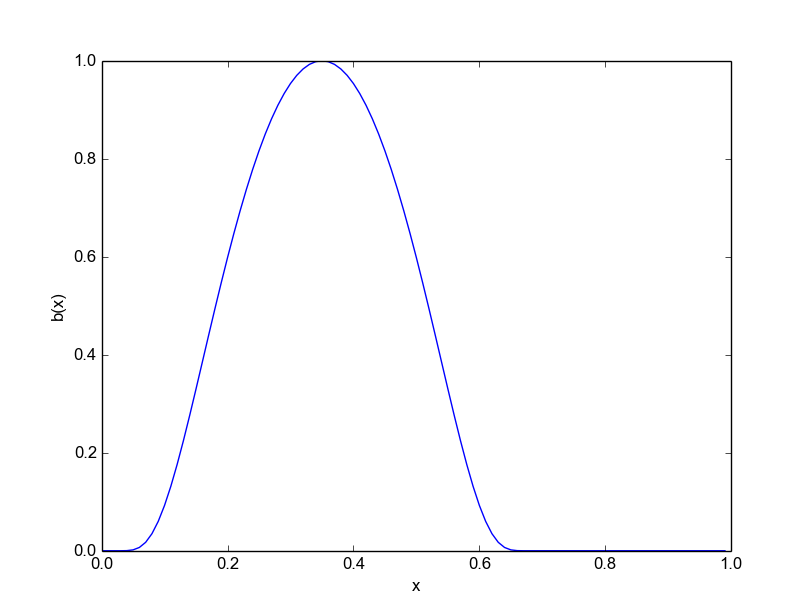
\includegraphics[width=10cm]{blip.png}
\caption{Graphe de la fonction $b_{(a,b)}(x)$, pour $(a,b)=(0;0,7)$ et avec $\alpha=0.4$.}
\end{center}
\end{figure}

Ainsi en utilisant cette fonction, nous avons défini un potentiel à deux dimensions qui a l'allure que l'on peut voir dans la Figure \ref{fig:potentiels}. 

\begin{figure}[h]
\centering
\begin{subfigure}{.5\textwidth}
	\centering
	\label{fig:pot}
	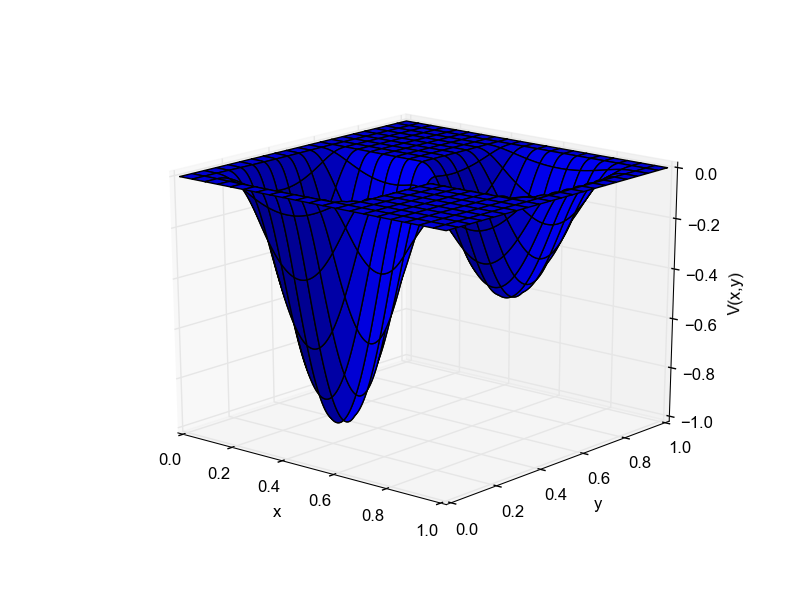
\includegraphics[width=10cm]{potentiel.png}
	\caption{Allure du potentiel $V(x,y)$.}
\end{subfigure}%
\begin{subfigure}{.5\textwidth}
	\centering	
	\label{fig:equipot}
	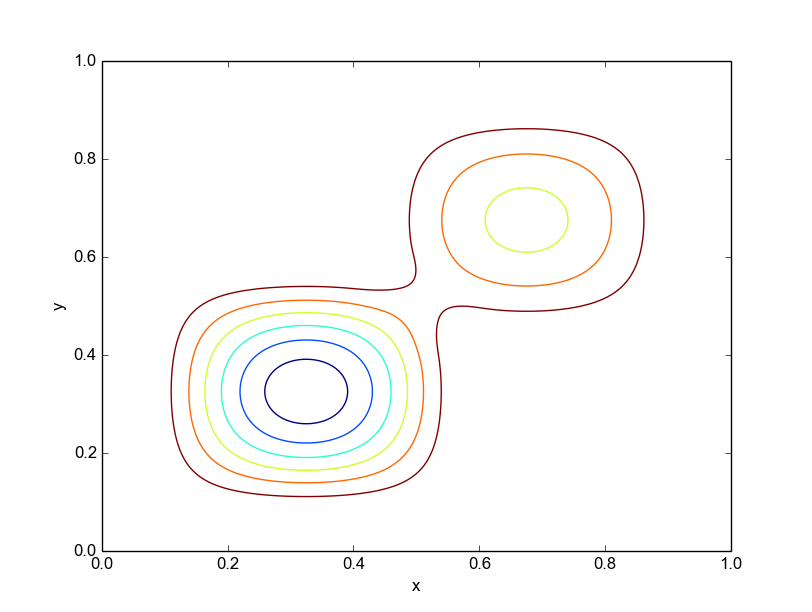
\includegraphics[width=10cm]{equipot.png}
	\caption{Allure des équipotentielles de $V(x,y)$.}
\end{subfigure}
\caption{Potentiel global utilisé ainsi que les équipotentielles.}\label{fig:potentiels}
\end{figure}

Enfin nous avons utilisé, lorsque nous avons simulé pour les deux particules, un potentiel d'intéraction $W(x_1,y_1,x_2,y_2)$ qui ne dépend que de la distance entre les deux particules (on prend le soin de bien définir la distance avec les conditions aux bords périodiques) qui est positif lorsque les deux particules sont proches et devient négatif lorsque la distance entre les deux particules est de l'ordre de la distance entre les deux puits du potentiel global. De cette manière, on espère que les deux particules seront dans des puits différentes. Le graphe de ce potentiel en fonction de la distance entre les deux particules est visible en Figure \ref{fig:inter}.

\begin{figure}[h]
\centering
\includegraphics[width=10cm]{wr.png}
\caption{Graphe du potentiel d'intéraction en fonction de la distance entre les deux particules.}\label{fig:inter}
\end{figure} 

Une fois le potentiel global et le potentiel d'interaction étant bien défini, nous avons défini, pour chaque particule, le schèma suivant. On note $X^{i}_t$ le vecteur qui donne la position de la $i_eme$ particule au pas de temps $t=k\Delta t$ où $\Delta t$ est le pas de temps et $k\in \mathbb{N}$ le nombre de pas faits.

Regardons d'abord comment simuler le système classique. Ainsi on définit un processus en posant : 
\begin{equation}
X^{i}_{t+1}=X^{i}_t-\vec{\nabla}V_{tot}(X^{i}_t,X^j_t)+\sigma \sqrt{\Delta t}\xi_t
\end{equation} 

Où on définit $\sigma =\frac{\sqrt{2}}{\beta}$, avec $\beta=\frac{1}{T}$ où $T$ est la température (on prend des unités naturelles où $k_B=1$. De même $\xi_t$ sont des variables gaussiennes i.i.d. de moyenne nulle et variance $1$. Il va de soi que $j\neq i$.

Chaque pas est accepté en utilisant l'algorithme de Métropolis que nous avons décrit plus haut.
\subsection{Path-Integral Monte-Carlo}



\newpage
\begin{thebibliography}{analytique}
\bibitem{Ceperley}D.M. Ceperley, \textit{Path integrals in the theory of condensed helium}, Reviews of Modern Physics, Vol. 67, No. 2, Avril 1995.
\bibitem{cances}Éric Cancès, Notes de Cours, M2 ANEDP.
\bibitem{feynman}R.P. Feynman, A.R. Hibbs, \textit{Quantum Mechanics and Path Integrals}, MacGraw Hill, 1965.
\bibitem{krauth} Werner Krauth, \textit{Statistical Mechanics : Algorithms and Computation}, MOOC disponible sur \href{http://coursera.org}, École Normale Supérieure. 
\end{thebibliography}
\end{document}